\cleardoublepage
\sectionnonum{附录一:重建算法Rust实现}

\begin{lstlisting}[language=Rust, style=boxed]
pub fn reconstruct(&self, mut ai: Vector3<f64>, mut ri: Matrix3<f64>) -> Result<Vec<Point>, &'static str> {
    let mut points = Vec::with_capacity(self.splines.len()); // define points vector and reserve capacity
    let mut alpha_last = 0.;
    for (ka, kb) in self.splines.iter().cloned() {
        if ka == 0. && kb == 0. {
            // ka == kb == 0, no rotation, only translation.

            // Ti vector, a translation vector.
            let ti = ri.pseudo_inverse(0.000000001)? * Vector3::new(0., 0., self.ds);

            // ai + ti, to get absolute coordinate of current point
            ai += ti;
            let slice = ai.column(0);
            // push absolute coordinate of current point
            // println!("(x, y, z): ({}, {}, {})", slice[0], slice[1], slice[2]);
            points.push(Point {
                x: slice[0] as f32,
                y: slice[1] as f32,
                z: slice[2] as f32,
            });
        } else {
            let k = (ka.powi(2) + kb.powi(2)).sqrt(); // composite curvature
            let theta = k * self.ds;
            let alpha = (ka / k).acos();
            let phi = alpha - alpha_last;
            alpha_last = alpha;

            let cos_phi = phi.cos();
            let sin_phi = phi.sin();
            let cos_theta = theta.cos();
            let sin_theta = theta.sin();


            ri = Matrix3::new(
                cos_phi, -sin_phi, 0.,
                sin_phi, cos_phi, 0.,
                0., 0., 1.,
            ) * ri;

            // get generalized inverse of ri; then dot product relative coordinate
            let ti = ri.pseudo_inverse(0.000000001)? * Vector3::new((1. - cos_theta) / k, 0., sin_theta / k);
            ai += ti;
            let slice = ai.column(0);
            // push absolute coordinate of current point
            // println!("(x, y, z): ({}, {}, {})", slice[0], slice[1], slice[2]);
            points.push(Point {
                x: slice[0] as f32,
                y: slice[1] as f32,
                z: slice[2] as f32,
            });

            ri = Matrix3::new(
                cos_theta, 0., sin_theta,
                0., 1., 0.,
                -sin_theta, 0., cos_theta,
            ) * ri;
        }
    }
    Ok(points)
}
\end{lstlisting}

\sectionnonum{附录二:最终软件展示}

\begin{enumerate}

\item \textbf{实时动态展示:\href{https://curve.hexilee.me:8000/}{https://curve.hexilee.me:8000/}}

\item \textbf{管壁渲染: 图 ~\ref{fig:tube-default}}

\item \textbf{管壁渲染,启用坐标轴: 图 ~\ref{fig:tube-with-axes}}

\item \textbf{管壁渲染,启用坐标轴和栅格: 图 ~\ref{fig:tube-with-axes-grid}}。

\item \textbf{轴线渲染: 图 ~\ref{fig:line}}。

\begin{figure}[H]
\centering
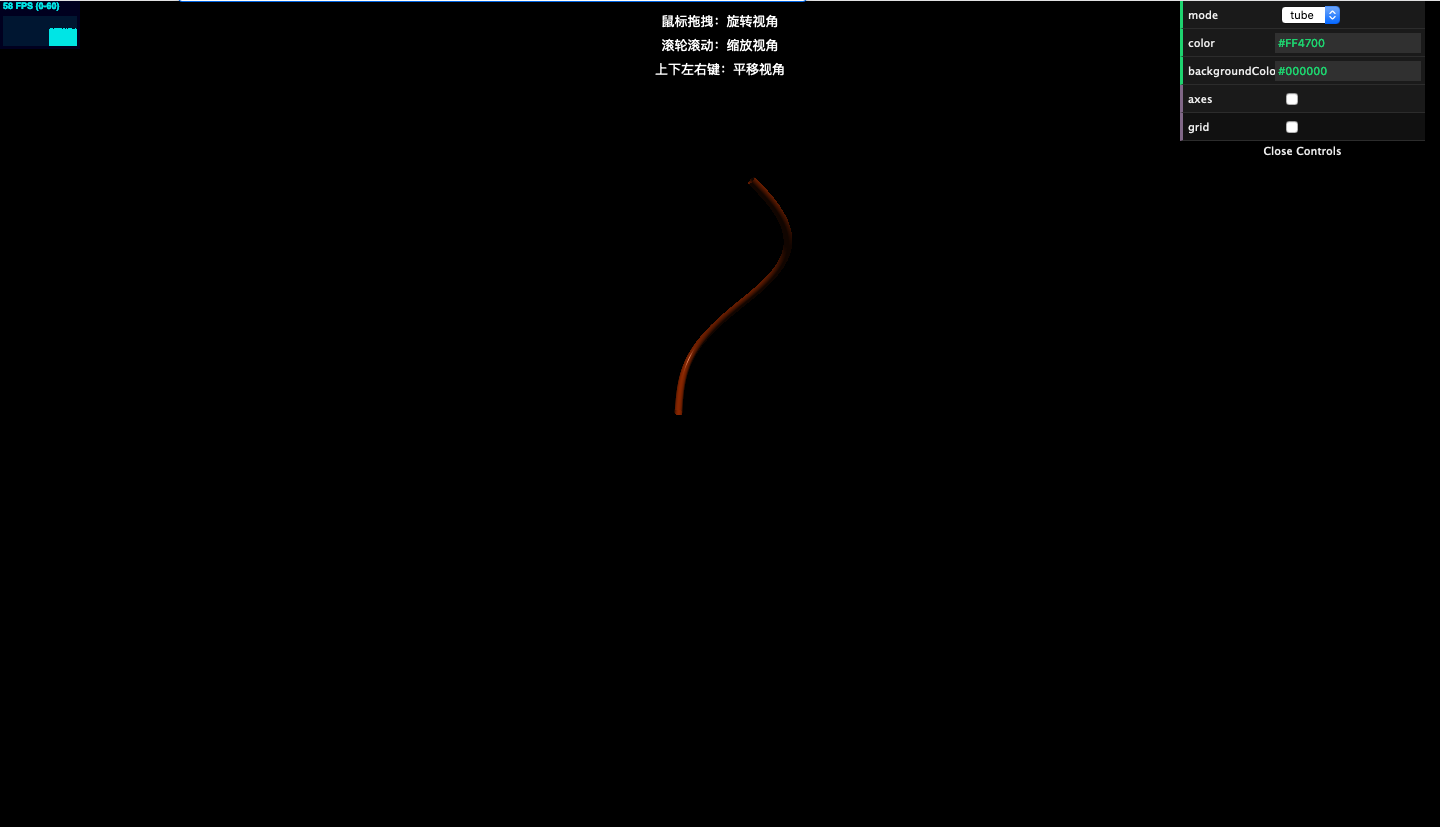
\includegraphics[scale=0.3]{tube-default.png}
\caption{管壁渲染}
\label{fig:tube-default}
\end{figure}

\begin{figure}[H]
\centering
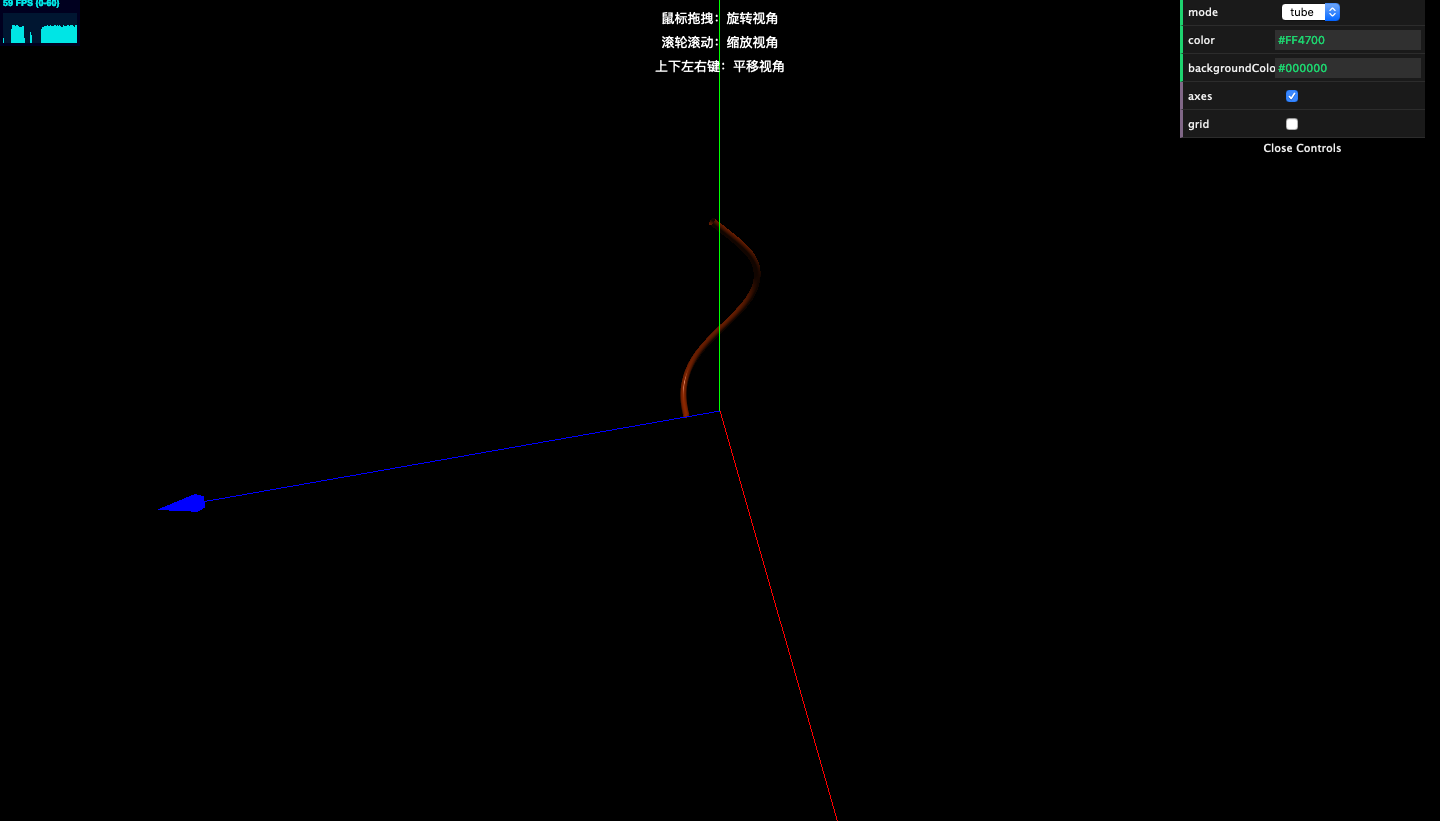
\includegraphics[scale=0.3]{tube-with-axes.png}
\caption{管壁渲染,启用坐标轴}
\label{fig:tube-with-axes}
\end{figure}

\begin{figure}[H]
\centering
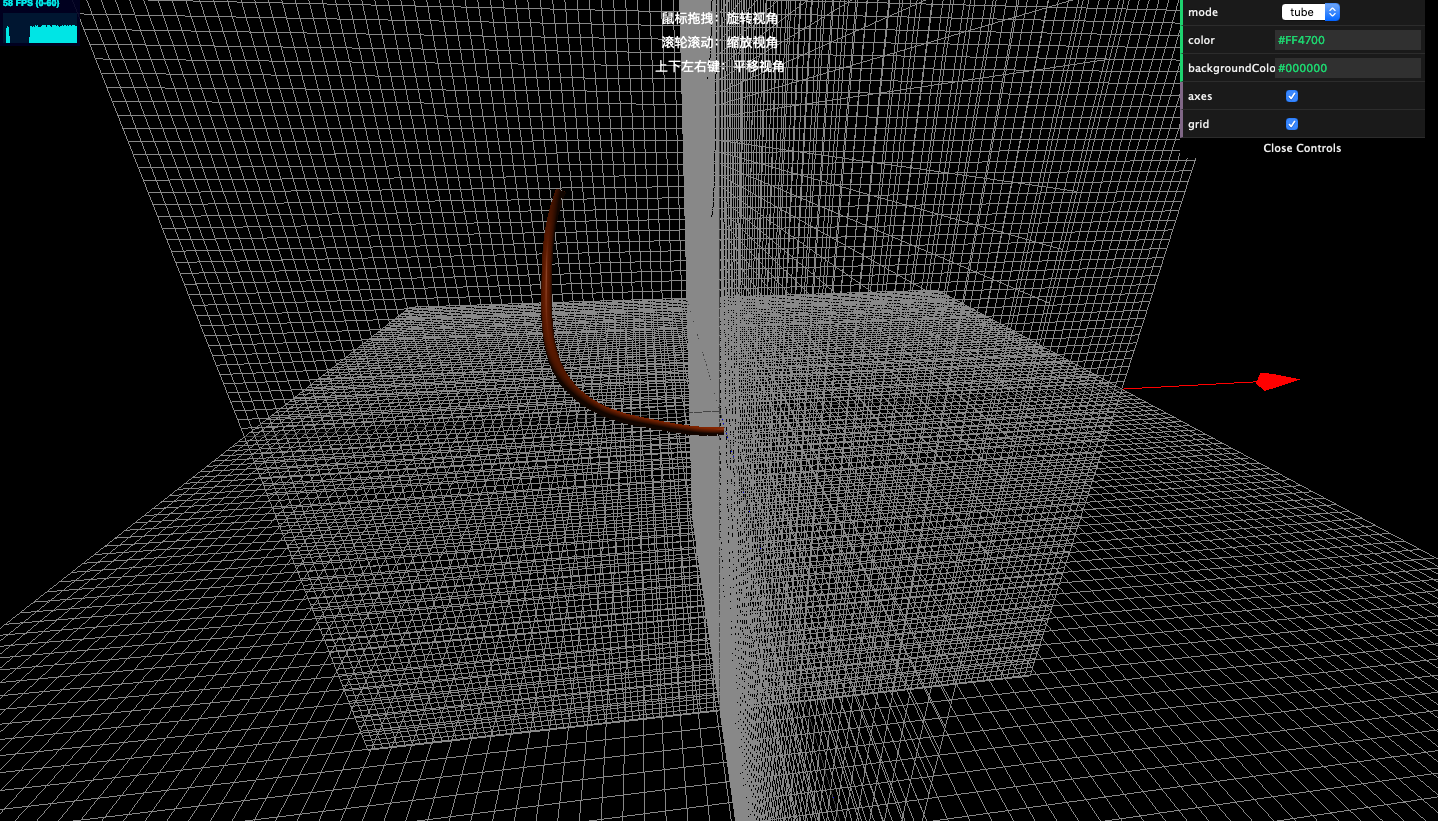
\includegraphics[scale=0.3]{tube-with-axes-grid.png}
\caption{管壁渲染,启用坐标轴和栅格}
\label{fig:tube-with-axes-grid}
\end{figure}

\begin{figure}[H]
\centering
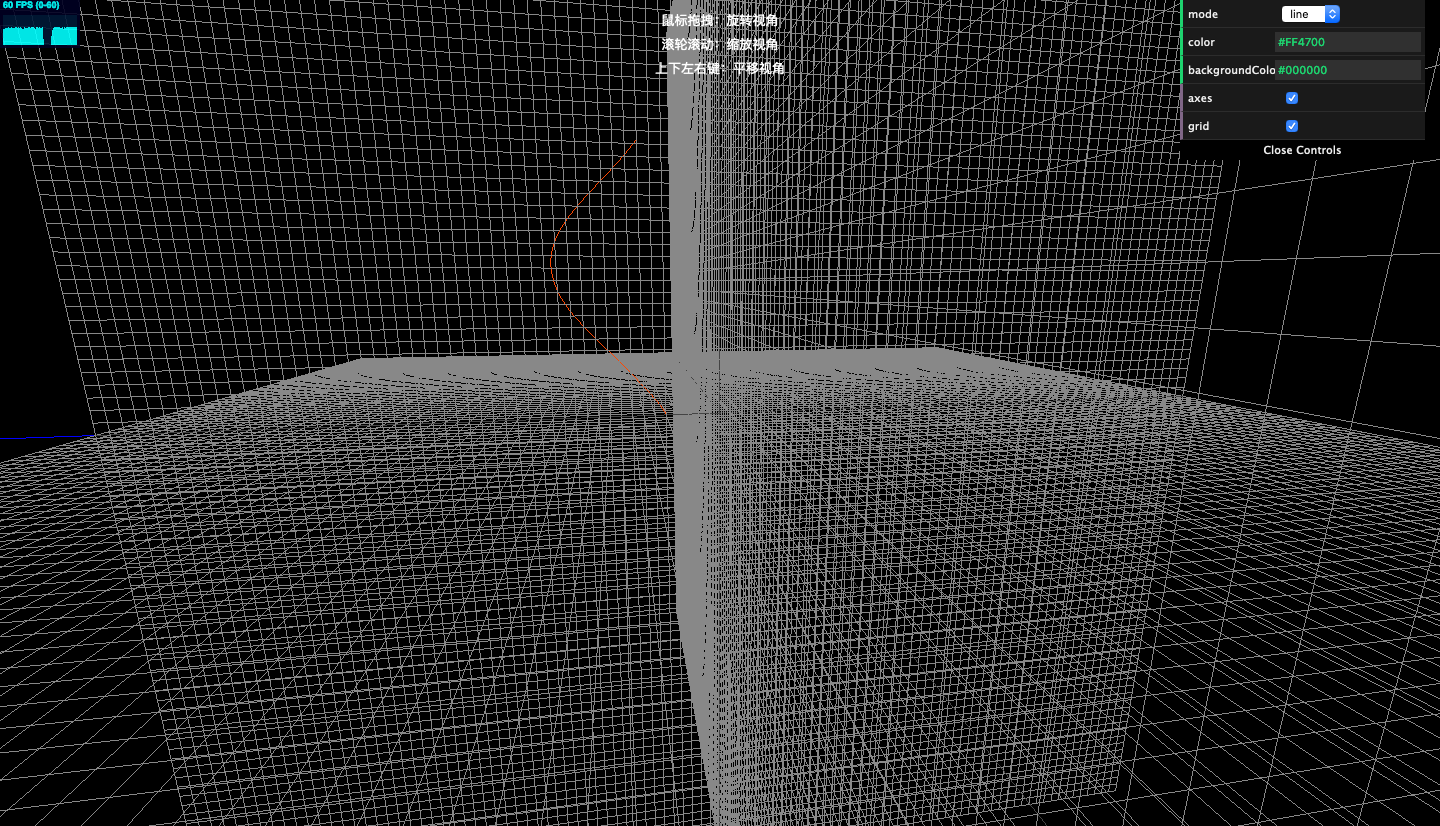
\includegraphics[scale=0.3]{line.png}
\caption{轴线渲染}
\label{fig:line}
\end{figure}

\end{enumerate}